\documentclass[a4paper, 12pt]{book}

% import pacchetti
\input{model/packages}

% definizione layout documento
\input{model/layout}

% Comandi ridefiniti
\input{model/new_commands}

% aggiunta bibliografia
\addbibresource{bib/bibliografia.bib}

\usepackage[italian]{babel}

% inizio documento
\begin{document}
	\renewcommand{\contentsname}{\vspace{-2cm} Indice \vspace{-0.5cm}}
	
	% FRONTESPIZIO	
	\begin{titlepage}
	
		\begin{center}
		
		 	% immagine sigillo unipd
			\includegraphics[scale=0.11]{images/sigillo.eps}
			\vspace*{1cm}
			
			\textsc{\LARGE Università degli Studi di Padova}\\
			\vspace{0.25cm}
			
			\textsc{\normalsize Dipartimento di Ingegneria dell'Informazione}\\
			\vspace{0.25cm}
			
			\textsc{\normalsize Corso di Laurea Triennale in Ingegneria Informatica}
			\vfill
			
			% Titolo
			\textsc{\LARGE Modifica della topologia di una rete neurale GRU e TCN}\\
			\vfill
			\vspace{4cm}
						
			% Relatore e Laureando
			\textsl{\large Relatore} \hfill \textsl{\large Laureando}\\
			\large Prof. Loris Nanni \hfill Riccardo Rampon
			\vfill
			
			% Data, AA
			{\large Anno Accademico 2020/2021}\\
			\textsl{\large Padova, 22 settembre 2021}				
		
		\end{center}
		
	\end{titlepage}
	
	\thispagestyle{empty} % pagina bianca dopo il titolo
	\cleardoublepage

	\clearpage{\pagestyle{plain}\cleardoublepage}
	\vspace*{\fill}
	\begin{flushright}
		\textit{A mamma, papà e Francesco}
	\end{flushright}
	\vspace*{\fill}
	
		
	% ABSTRACT ----------------------------------------------------------------------------
	\clearpage{\pagestyle{plain}\cleardoublepage}
	\chapter*{Abstract} % nome capitolo
	\label{chapter:zero}
	\addcontentsline{toc}{chapter}{Abstract}
	L'apprendimento Multi-label è una delle classi di apprendimento che ammette per ogni istanza l'assegnazione di più più labels contemporaneamente. Il lavoro su cui è basato questo elaborato propone un nuovo insieme di metodi per la classe di problemi rappresentata dalla classificazione Multi-label, nei quali il nucleo dell'approccio proposto prevede di combinare tra loro un insieme di Gated Recurrent Units (GRU) e Temporal Convolutional Neural Networks (TCN) con l'utilizzo di una nuove varianti rispetto al metodo di ottimizzazione Adam (Adaptive Momentum stimation). Inoltre, le reti neurali proposte vengono combinate con l'approccio IMCC (Incorporating Multiple Clustering Centers) che rappresenta l'attuale stato dell'arte in merito alla classificazione Multi-label. Gli esperimenti effettuati dimostrano la potenza di questo approccio, che ha dimostrato di superare i migliori metodi riportati in letteratura. % importa il capitolo dal corrispondente file
	
	\pagenumbering{gobble} 
	\thispagestyle{empty}
	\clearpage{\pagestyle{plain}\cleardoublepage}
	\tableofcontents %Indice
	
	\clearpage{\pagestyle{plain}\cleardoublepage} %Numerazione araba per i capitoli
	\pagenumbering{arabic}

	% INTRODUZIONE -------------------------------------------------------------------------
	\clearpage{\pagestyle{plain}\cleardoublepage} % inizia il nuovo capitolo su di una pagina dispari
	\chapter{Introduzione} % nome capitolo
	\label{chapter:primo} % label capitolo
	\addcontentsline{toc}{chapter}{Introduzione}
	\section{Intelligenza artificiale}
% Cos'è l'intelligenza artificiale
\cite{boutell2004learning}
L'intelligenza artificiale, dall'inglese \textit{Artificial Intelligence} (abbreviato in AI), è una disciplina appartenente all'informatica che studia i fondamenti teorici, le metodologie e le tecniche che consentono la programmazione e progettazione di sistemi hardware e software che permettono di dotare gli elaboratori elettronici di determinate caratteristiche che vengono considerate tipicamente umane quali, ad esempio, le percezioni visive, spazio-temporali e decisionali; sono capaci, dunque, di riprodurre parzialmente l'attività intellettuale umana. In particolare, è considerato un comportamento intelligente quello di un programma che apprende dall'esperienza al fine di migliorare le sue prestazioni nella risoluzione di un task.
\section{Deep-Learning}
% Deep Learning
L'approccio più moderno e soprattutto più recente adottato nell'implementazione di intelligenze artificiali è quello dell'\textit{apprendimento profondo} (in inglese Deep Learning) che consiste in un insieme di tecniche basate su reti neurali artificiali composte da molti livelli organizzati gerarchicamente, nel quale ogni livello calcola i valori per quello successivo affinché l'informazione venga elaborata in maniera sempre più completa.

% Reti neurali
Una \textit{rete neurale artificiale} è un modello computazionale composto da neuroni artificiali, definiti come modello matematico, che si ispirano vagamente al funzionamento dei neuroni biologici e alla struttura di una rete neurale biologica.

\section{Recurrent Neural Network}
Una parte del lavoro svolto riguarda un categoria particolare di reti neurali: la reti neurali ricorrenti (in inglese Recurrent Neural Network o abbreviato RNN).
La caratteristica principale di questa tipologia di rete è prevedere delle connessioni di feedback (in genere verso neuroni dello stesso livello, ma anche "all'indietro"). Questo ne complica notevolmente il flusso di informazioni e la fase di addestramento, in quanto è richiesta la considerazione del comportamento della rete in più istanti temporali. Questo tipo di rete è particolarmente indicata quando si lavora con pattern che rappresentano sequenze, perché dotate di un effetto memoria (di breve termine) che al tempo t rende disponibile l'informazione processata al tempo t-1,t-2 e così via. 

Un ruolo fondamentale nella costruzione di una rete neurale ricorrente viene svolto dalle celle, che possiamo considerare come delle componenti principali. La cella è la parte della rete ricorrente che ha uno stato (o memoria) $h_{(t)}$ al suo interno per ogni istanza temporale. E' costituita da un numero prefissato di neuroni (di fatto può essere vista come un layer della rete). Lo stato $h_{(t)}$ dipende dall'input $x_{(t)}$ e dallo stato precedente $h_{(t-1)}$:
\begin{equation}
	h_{(t)} = f(h_{(t-1)}, x_{(t)})
\end{equation}
Esistono diverse tipologie di celle che differiscono principalmente per la loro struttura e per come trattano lo stato di memoria $h_{(t)}$; un esempio sono le Long-Short Term Memory (LSTM) e le Gated Recurrent Unit (GRU). Quest'ultima tipologia sarà utilizzata nel metodo proposto e nelle varianti topologiche dell'elaborato.

\begin{comment}
% Obiettivo tesi: modifica della topologia di una rete neurale
L'oggetto principale del presente studio è stata la modifica della topologia di due reti neurali artificiali, nello specifico di una rete neurale ricorrente (in inglese \textit{Recurrent Neural Netowrk} o abbreviato RNN) con cella GRU (Gated Recurrent Unit) e di una TCN (Temporal Convolutional Neural Network). Un altro argomento presente è stata la trattazione di diverse \textit{feature transform} per la gestione di un dataset altamente sparso.

% Organizzazione dell'elaborato
La stesura di questo elaborato è stata articolata in quattro capitoli. Inizialmente, verranno brevemente esposti alcuni concetti teorici rilevanti nel contesto delle modifiche svolte. La trattazione proseguirà con la presentazione delle modifiche effettuate e delle feature trasform individuate e le relative performance. Infine, verranno tratte delle conclusioni riguardo il lavoro svolto.

% MATLAB come linguaggio di programmazione % da aggiungere (vedi IVANCHIC)
Tutto il codice sviluppato il relazione a questo lavoro è stato scritto in MATLAB, un ambiente per il calcolo numerico e l'analisi statistica scritto in linguaggio di programmazione C.
\end{comment}

\section{Multi-label}
L'apprendimento Multi-label è una delle classi di apprendimento che ammette per ogni istanza l'assegnazione di più etichette contemporaneamente. Grazie alla particolarità di poter far fronte a oggetti del mondo reale con molteplici significati semantici, l'apprendimento Multi-label può essere utilizzato in diversi domini applicativi che spaziano dal tag recommendation alla bioinformatica, dall'information retrieval al rule mining, web mining e molti altri.

In questo elaborato vengono proposte due modifiche di topologie di reti neurali basate su un nuovo insieme di metodi per la classificazione Multi-label, nei quali la parte centrale è data dalla combinazione di insiemi di Gated Recurrent Units (GRU) e Temporal Convolutional Neural Networks (TCN). Ogni ensemble è sviluppato usando approcci di ottimizzazione differenti, che permettono un aumento delle performance e un rimescolamento delle features per ogni rete rispetto all'uso del metodo Adam orginale. 

Inoltre, un ulteriore miglioramento delle prestazioni è ottenuto combinando tra loro i set proposti di GRU e TCN con lo stato dell'arte per la classificazione Multi-label, Incorporating Multiple Clustering Centers.

\section{Datasets}
Per valutare i diversi ensemble creati occorrono datasets con categorizzazione multi-label binaria. Sono stati utilizzati nove datasets basati su domini applicativi molto differenti tra loro (image classification, musica, biologia, farmaci):

\begin{itemize} %%%%%%% CITARE OGNI DATASET

	\item Cal500 è un dataset musicale composto da 502 canzoni rappresentate da 68 feature numeriche. Ogni istanza è stata annotata manualmente da annotatori umani utilizzando 174 etichette distinti. Queste etichette sono divise in 6 categorie semantiche: strumentazione, caratteristiche vocali, generi, emozioni, qualità acustica e termini d'uso.
	
	\item Image è un dataset composto da 2000 immagini. Nello specifico ogni immagine a colori viene prima convertita nello spazio CIELUV, che è uno spazio colore più percettivamente  uniforme in modo tale che le differenze di colore percepite corrispondano esattamente alle di corrispondano strettamente alle distanze euclidee.Successivamente, l'immagine viene divisa in 49 blocchi utilizzando una griglia 7×7, in cui in ciascun blocco viene calcolata la media e la varianza di ogni banda. Infine, ogni immagine viene trasformata in un feature vector 49×3×2 = 294-dimensionale. 
	
	\item Scene (citare) è un dataset etichettato di immagini per la classificazione multipla di scene. Include 2407 istanze rappresentate da 294 feature numeriche e 6 etichette distinte.
	
	\item Yeast (citare) è un dataset biologico che include 2417 micro-array di dati e profili filogenetici. Ogni istanza viene rappresentata da 103 feaure numeriche e 14 etichette distinte. 
	
	\item Arts (citare) è un dataset costituito da 5000 immagini artistiche, ciascuna descritta da 462 feature numeriche in cui ogni immagine può appartenere ad alcune delle 26 classi presenti.
	
	\item ATC (citare) è una raccolta di 3883 prodotti farmaceutici codificati Anatomical Therapeutic Chemical (ATC). Ogni istanza è rappresentata da 42 feature e 14 classi.
	
	\item ATC-f (citare) è una variante della raccolta citata sopra che include le stesse istanze, ma rappresentate da un descrittore 806-dimensionale.
		
	\item Liu (citare) è un dataset di farmaci raccolti per prevedere in silico i loro effetti collaterali. Comprende 832 farmaci rappresentati da 2892 feature e 1385 etichette.
	
	\item mAn (citare) è una dataset di proteine rappresentate da 20 feature e 20 etichette.
	
\end{itemize}

Il dataset di riferimento per questo elaborato è il dataset \textit{Liu} che costituisce un insieme di farmaci raccolti per prevedere in silico i loro effetti collaterali.

\vspace{0.25cm}

% tabella riassuntiva
\begin{table}[h!]
	\begin{center}
	\begin{tabular}{|| c | c | c | c ||} 
 	\hline
	\textbf{Nome} & \textbf{n° patterns} & \textbf{n° features} & \textbf{n° etichette} \\
	\hline
	CAL500 & 502 & 68 & 174 \\
	\hline
	Image & 2000 & 294 & 5 \\
	\hline
	Scene & 2407 & 294 & 5 \\
	\hline
	Yeast & 2417 & 103 & 14 \\
	\hline
	Arts & 5000 & 462 & 26 \\
	\hline
	ATC & 3883 & 42 & 14 \\
	\hline
	ATC-f & 3883 & 700 & 14 \\
	\hline
	Liu & 832 & 2892 & 1385 \\
	\hline
	mAn & 3916 & 20 & 20 \\
	\hline
	\end{tabular}
	\caption{Riepilogo dataset}
	\label{Tabella 1}
	\end{center}
\end{table}

\newpage
\section{Indicatori di performance}
La classificazione multi-label viene valutata utilizzando diversi indicatori di performance utili per poter confrontare i risultati ottenuti con quelli della Incorporating Multiple Clustering Centers (IMCC), stato dell'arte per la classificazione multi-label. Sia X un insieme di dati che include \textit{m} campioni $x_{i} \in \Re^{d}$ ciascuno avente un'etichetta $y_{i} \in \{0,1\}^{l}$, dove \textit{l} è il numero di etichette. Siano H, F l'insieme di etichette predette, dove $h_{i} \in \{0,1\}^l$ è il vettore dell'etichetta predetta rispetto al campione $x_{i}$ e $f_{i} \in \Re^{l}$ è il valore di confidenza di ciascuna previsione.
I seguenti indicatori di prestazione possono essere definiti per H, F:

\begin{itemize}

	\item Hamming Loss, è il rapporto fra le etichette classificate erroneamente e il numero totale di etichette,
	\begin{equation}
		HLoss(H) = \frac{1}{ml}\sum_{i=1}^{m}\sum_{j=1}^{l}I(y_{i}(j)\neq h_{i}(j))
	\end{equation}
	dove $I()$ è la funzione indicatrice. Hamming Loss è una \textit{loss function}, dunque il suo valore ottimo è 0 e il suo upper-bound è 1. Deve essere minimizzata: se il valore dell'hamming loss è 0 allora non sono presenti errori nel vettore dell'etichette predette.
		
	
	\item One error, è il rapporto tra le istanze le cui etichette con il più alto livello di confidenza sono classificate erroneamente, deve essere minimizzato:
	\begin{equation}
		OneError(F) = \frac{1}{m}\sum_{i=1}^{m}I(h_{i}(arg\max_{j}f_{i}) \neq y_{i}(arg\max_{j}f_{i}))
	\end{equation}
	dove $I()$ è la funzione indicatrice.
	
	\item Ranking loss, è il rapporto medio delle coppie di etichette ordinate in modo contrario  per ciascuna istanza. Può essere ottenuto dal valore di confidenza, considerando il numero di confidenze tra coppie di etichette correttamente classificate (cioè un'etichetta classificata correttamente ha un ranking migliore rispetto ad una classificata erroneamente). Ranking loss è una \textit{loss function} e dunque deve essere minimizzato.
	
	\item Coverage, è il numero medio di step necessari per spostarsi in basso nella lista delle etichette classificate di una istanza in modo tale da coprire tutte le relative etichette. Dovrebbe essere minimizzato.
	
	\item Average precision, è il rapporto medio delle etichette con classificate in modo migliore rispetto ad una particolare etichetta. Deve essere massimizzato.	
	
	\item Aiming, è il rapporto tra le etichette correttamente predette e le tutte le etichette previste:
	\begin{equation}
		Aiming(H) = \frac{1}{m}\sum_{i=1}^{m}\frac{||h_{i}\cap y_{i}||}{||h_{i}||}
	\end{equation}
	
	\item Recall, valuta quante etichette "positive" sono state effettivamente classificate, indica quanto il sistema è selettivo:
	\begin{equation}
		Recall(H) = \frac{1}{m}\sum_{i=1}^{m}\frac{||h_{i}\cap y_{i}||}{||y_{i}||}
	\end{equation}
	
	\item Accuracy, è la percentuale media di etichette correttamente predette rispetto alle etichette totali:
	\begin{equation}
		Accuracy(H) = \frac{1}{m}\sum_{i=1}^{m}\frac{||h_{i}\cap y_{i}||}{||h_{i}\cup y_{i}||}
	\end{equation}
	
	\item Absolute true, è la percentuale delle etichette correttamente predette rispetto alle previsioni totali:
	\begin{equation}
		AbsTrue(H) = \frac{1}{m}\sum_{i=1}^{m}I(h_{i} == y_{i})
	\end{equation}
	
	\item Absolute false, è la percentuale delle previsioni errate rispetto alle previsioni totali:
	\begin{equation}
		AbsFalse(H) = \frac{1}{m}\sum_{i=1}^{m}\frac{||h_{i}\cup y_{i}||-||h_{i}\cap y_{i}||}{l}
	\end{equation}
	
\end{itemize}


 % importa il capitolo dal corrispondente file
	
	% APPROCCIO PROPOSTO -------------------------------------------------------------------------
	\clearpage{\pagestyle{plain}\cleardoublepage} % inizia il nuovo capitolo su di una pagina dispari
	\chapter{Approccio proposto} % nome capitolo
	\label{chapter:secondo} % label capitolo
	\addcontentsline{toc}{chapter}{Approccio proposto}
	In questo paragrafo viene introdotto con più dettagli il metodo proposto.
\section{Architettura del modello}
È stata creata un'architettura Deep Neural Network (DNN) basata su Gated Recurrent Unit (GRU) e Temporal Convolutional Neural Network (TCN) entrambe adattate al problema della classificazione multi-label. Il primo modello proposto, visibile in \ref{Figura 1.}, presenta una GRU con H unità nascoste (il numero H di unità nascoste è impostato a 50 nel nostro caso), seguito da un livello di max-pooling, da uno fully-connected e da un livello di output  sigmoid. L'approccio proposto per la TCN è il medesimo, con la differenza che il livello di max-pooling viene posto dopo il fully-connected.
\vspace{0.25cm} 
\begin{center}
	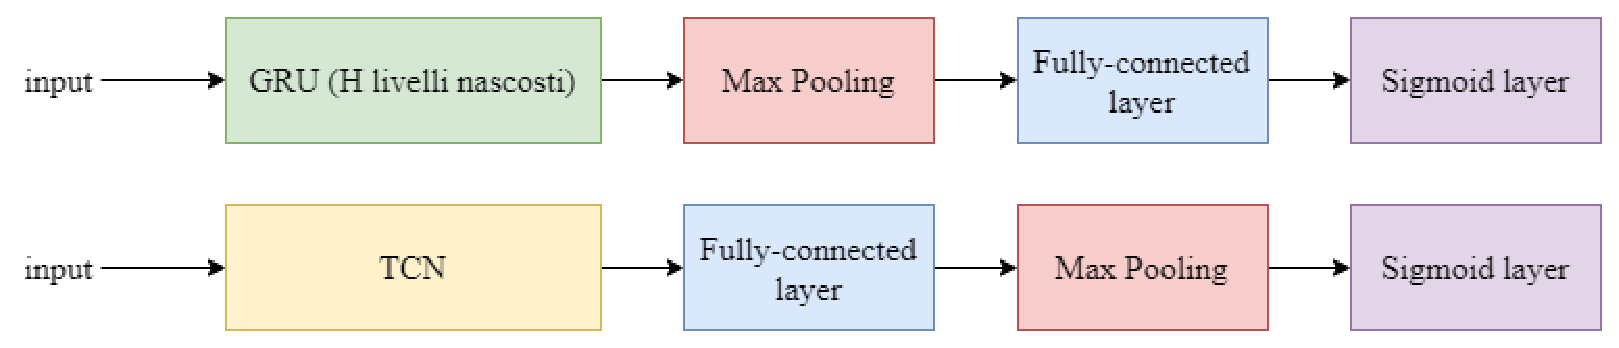
\includegraphics[scale=0.55]{images/arch.eps} %correggere GRU(H UNITA' nascoste)
	\captionof{figure}{Schema della DNN ricorrente}
	\label{appr:dnn}
\end{center}
\vspace{0.25cm}
Come \textit{loss function} è stata utilizzata la Binary Cross-Entropy calcolata dalle etichette predette e dalle etichette "obiettivo" (target-labels). La Binary Cross-Entropy calcola la perdita di una insieme di $ m $ osservazioni calcolando la seguente media:
\begin{equation}
	CELoss = -\frac{1}{m}\sum_{i=1}^{m}\sum_{j=1}^{l}y_{i}(j)\cdot\log(h_{i}(j))+(1-y_{i}(j))\cdot\log(1-h_{i}(j)) 
\end{equation}
dove $y_{i} \in \{0,1\}^l$ sono le etichette associate ad una istanza e $h_{i} \in \{0,1\}^l$  è il vettore delle etichette predette rispettivamente a ciascuna istanza.

\section{Pre-Processing}
Sebbene in molti problemi non si richiede un pre-processing dei dati d'input, ovvero una loro pre-elaborazione, prima di essere classificati tramite reti GRU, molto spesso invece questa è necessaria nel momento in cui tali dati sono feature vector che assumono valori con alta varianza. 

Il dataset di riferimento per questo elaborato è il dataset \textit{Liu}, che costituisce un collezione di farmaci raccolti per prevedere in silico i loro effetti collaterali. Una particolarità di questo dataset è il fatto che è estremamente sparso e ciò lo si può notare dal numero di features utilizzate per rappresentare ciascun pattern e il numero di etichette possibili. Un dataset che ha una tale peculiarità può rappresentare un problema soprattutto per la presenza dell'\textit{over-fitting}, ovvero una situazione in cui, a causa degli elevati gradi di libertà, il classificatore raggiunge un'elevata accuratezza sul Training-set, ma non sul Test-set e ciò lo porta ad "imparare a memoria" e a non generalizzare la predizione nel mondo reale.

Per evitare tale problematica è stata eseguita una riduzione di dimensionalità utilizzando diverse feature transform come PCA (Principal Component Analysis), t-SNE (t-Distributed Stochastic Neighbor Embedding) e KPCA (Kernel Principal Component Analysis).

\section{PCA}
forse spiego

\section{t-SNE}
forse spiego

\section{KPCA}
forse spiego

\section{Gated Recurrent Unit}
Gated Recurrent Unit (GRU) rappresenta una delle diverse tipologie di cella presente nelle reti neurali ricorrenti, introdotte nel 2014 da Kyunghyun Cho et al. (cita). GRU mira a risolvere principalmente il problema del vanishing (o exploding) gradient ovvero la scomparsa del gradiente. 

Tale problematica di sviluppa su reti neurali profonde e ne crea una difficoltà nell'addestramento tramite retro-propagazione dell'errore (backpropagation). Una delle principali cause è l'utilizzo di funzioni di attivazione non lineari standard, come la sigmoide, la tangente iperbolica o la funzione logistica, che sono caratterizzate dall'avere il gradiente a valori nell'intervallo $[0,1]$; ciò porta, nell'applicazione della regola di derivazione a catena, a far decrescere esponenzialmente i valori dei parametri del modello nei livelli lontani dall'output. Si dice che tali funzioni hanno un comportamento di tipo saturante.

La cella GRU può essere considerata come una variante semplificata della cella LSTM (Long-Short Term Memory) che cerca di mantenerne i vantaggi, riducendo parametri e complessità. Rispetto alla LSTM, GRU presenta un forget gate che permette alla rete di decidere quale parte della vecchia informazione è rilevante per comprenderne la nuova.

% prestazioni
GRU fornisce prestazioni simili a LSTM in problemi come lo speech signal modeling, polyphonic music modeling e natural language processing (citazione 11-12). Secondo (citazione 13-14) le celle GRU hanno prestazioni migliori su dataset di piccole dimensioni.

\vspace{0.25cm} 
\begin{center}
	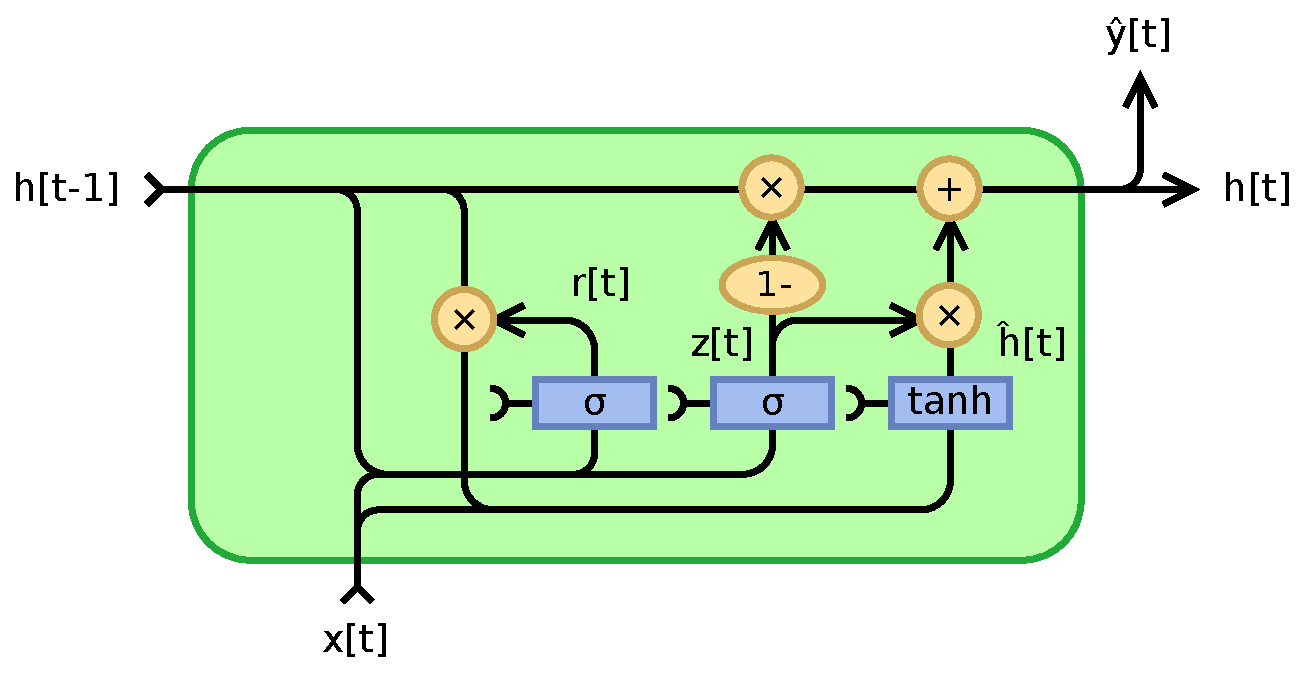
\includegraphics[scale=0.4]{images/gru2.eps}
	\captionof{figure}{Struttura di una cella GRU}
	\label{Figura 1.}
\end{center}
\vspace{0.25cm}

%componenti gru
Le componenti fondamentali di una cella GRU sono il reset gate e l'update gate: il primo determina quanta della passata informazione dimenticare mentre il secondo quale informazione può essere dimenticata e quale passata all'output. 

Sia $x_{t}$ la sequenza di input e $h_{t}$ quella di output; inizializziamo $h_{0}=0$ come lo stato di memoria della cella nell'istante $t=0$. Definiamo l'update gate vector $z_{t}$ e il reset gate vector $r_{t}$ come
\begin{equation}
	z_{t} = \sigma(W_{z}x_{t}+U_{z}h_{t-1}+b_{z}) 
\end{equation}
\begin{equation}
	r_{t} = \sigma(W_{r}x_{t}+U_{r}h_{t-1}+b_{r})
\end{equation}
dove $W_{z}$, $U_{z}$, $b_{z}$, $W_{r}$,$U_{r}$, $b_{r}$ sono parametri matrici e vettori e $\sigma$ è la funzione sigmoidea. 

Definiamo
\begin{equation}
	\hat{h_{t}} = \phi(W_{h}x_{t}+U_{h}(r_{t} \bigodot h_{t-1})+b_{h})
\end{equation}
come l'activation vector candidato, dove $\phi$ è la funzione di attivazione tangente iperbolica e $\bigodot$ è l'Hadamard product (o component-wise product).
Sapendo che il parametro $r_{t}$ determina la quantità di informazione passata che è rilevante per l'activation vector candidato, si ha che
\begin{equation}
	h_{t} = (1-z_{t}) \bigodot h_{t-1}+z_{t} \bigodot \hat{h_{t}} 
\end{equation}
è l'output vector, che va a rappresentare lo stato di memoria della cella nell'istante $t$.

\section{Temporal Convolutional Neural Network}
Le Temporal Convolutional Neural Network (TCN) (citazione?) sono una classe di reti neurali che sfrutta una gerarchia di convoluzioni per estrarre informazioni da sequenze di input o da serie temporali.
Generalmente i problemi legati alle serie temporali sono risolti da architetture di reti neurali ricorrenti (RNN) che, come sappiamo, introducono un modo per poter conservare e memorizzare l'informazione, ma Bai et al. \textbf{(citazione)} dimostra come reti neurali convoluzionali (CNN) possono eguagliare o addirittura superare le prestazioni delle reti ricorrenti.

La caratteristica più rilevante delle TCN è che utilizzano dei livelli convolutivi 1D impilati l'uno sull'altro per creare una rete profonda, utili poter eseguire la convoluzione sulla dimensione temporale.

Oltretutto, ognuno di questi livelli possiede un fattore di dilatazione (dilation factor) che aumenta esponenzialmente man mano che la rete diventa profonda, consentendo ai primi livelli di cercare informazioni molto vicine tra loro temporalmente e ai livelli più profondi di individuare dipendenze a lungo termine, in base alla feature estratta dai livelli precedenti. Ciò consente alle reti TCN ti avere un \textit{reciptive field} molto ampio, superando di fatto uno dei limiti presenti nelle architetture RNN. 

La dimensione del \textit{reciptive field} può essere calcolata come segue:
\begin{equation}
	R = (f-1)(2^K-1)+1
\end{equation}
dove $f$ è la dimensione del filtro usato nelle convoluzioni e $K$ è il numero di livelli convoluzionali.

Il \textit{fattore di dilatazione} delle convoluzioni è $2^{(k-1)}$, dove $k$ è il numero di livelli convoluzionali.

\vspace{0.25cm} 
\begin{center}
	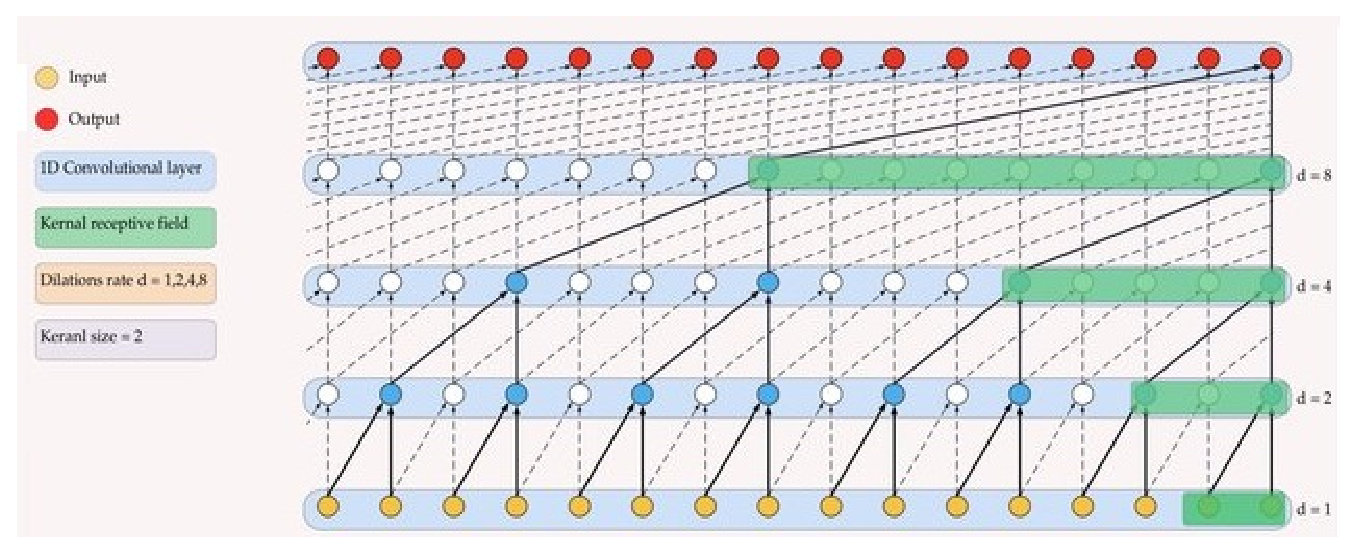
\includegraphics[scale=0.7]{images/esempio_tcn_dilatation.eps}
	\captionof{figure}{Esempio di struttura interna di una TCN, dove $d$ è il \textit{dilatation factor}}
	\label{Figura 1.}
\end{center}
\vspace{0.25cm}

% architettura tcn
L'architettura della TCN utilizzata nell'elaborato è formata da 4 blocchi, chiamati \textit{residual block}; ciascun blocco è costituito da due set ognuno dei quali comprende un livello convoluzionale dilatato casualmente, con 175 diversi filtri di dimensione $3x3$, seguito da un livello di attivazione ReLU, da un livello di Batch normalization e da un livello di Spatial dropout. L'input di ciascun blocco viene poi aggiunto all'output dello stesso (incluso un livello convoluzionale 1-by-1 opzionale, che si aggiunge quando il numero di canali tra l'input e l'output non coincidono).

Inoltre è stato utilizzato un livello fully-connected seguito da un livello di max-pooling ed, infine, come livello di output è stato utilizzato uno sigmoideo per ottenere la classificazione multiclasse.

Per l'addestramento è stato utilizzato un \textit{dropout factor} con probabilità 0.05.

\section{Pooling}
Dopo il nucleo principale della rete GRU/TCN è stato inserito un livello di Pooling, con lo scopo di ridurre la dimensionalità dei dati processati mantenendo solo l'informazione più rilevante e facendo diminuire la probabilità di overfitting, problema già accennato nell'introduzione. In particolare è stato utilizzato un livello di max-pooling lungo la dimensione temporale.

\section{Livello fully-connected e livello sigmoideo}
I livelli Fully-connected (o completamente connessi) in una rete neurale sono quei livelli in cui tutti gli input di un livello sono collegati a ogni unità di attivazione del livello successivo. Nei modelli di apprendimento  automatico più diffusi, gli ultimi livelli sono tipicamente completamente connessi, che hanno lo scopo di compialre i dati estratti dai livelli precedenti per formare l'output finale della rete. È il secondo livello più dispendioso in termini di tempo, dopo il livello Convoluzionale.
Il livello Fully-connected è composto da $l$ neuroni ($l$ è il numero di etichette di output di un dato problema) completamente connessi con i livelli precedenti. È stata utilizzata una funzione sigmoidea come funzione di attivazione nel livello finale in modo da riportare un valore di attivazione nell'intervallo $[0...1]$, che può essere interpretato come valore finale di probabilità per ogni etichetta. 

Pertanto, l'output del modello è un vettore di classificazione multi-label: l'output di ciascun neurone del livello fully-connected fornisce una votazione (che varia da 0 a 1) per una singola etichetta.

\vspace{0.25cm} 
\begin{center}
	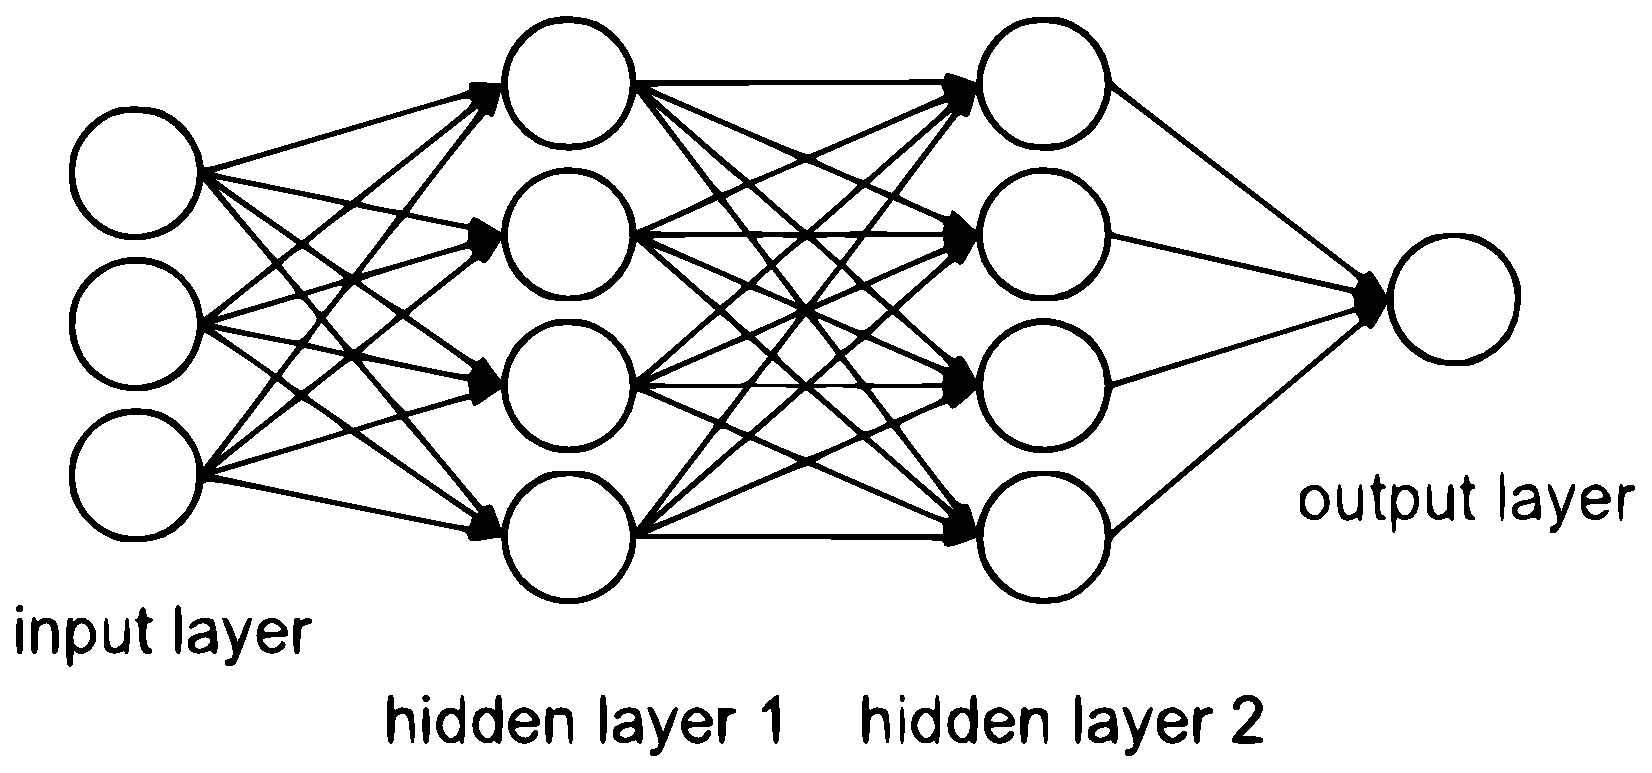
\includegraphics[scale=0.4]{images/neural_net2.eps}
	\captionof{figure}{Esempio di fully-connected layer}
	\label{Figura 1.}
\end{center}
\vspace{0.25cm}

\section{Addestramento}
L'addestramento viene eseguito utilizzando diverse varianti del metodo di ottimizzazione Adam che verranno presentate nel capitolo 5. È stato utilizzato un learning rate piuttosto alto pari a 0.01, un gradient decay di 0.5 e un squared gradient decay di 0.999.

Un altro passaggio effettuato è stato clippare il gradiente con una soglia pari a 1 utilizzando la L2-norm.

La dimensione di ciascun mini-batch è stata fissata a 30, mentre il numero di epoche è stato settato a 150 per GRU e 100 per TCN.

\section{Creazione degli ensemble}
Gli ensemble combinano l'output di più modelli per migliorare le prestazioni del sistema e contrastare l'overfitting. Un buon metodo per migliorare le previsioni e la generalizzazione dell'ensemble è aumentare la diversità dei classificatori. L'architettura degli ensemble è basata sulla fusione con average rule di diversi modelli addestrati sullo stesso problema. 

Gli ottimizzatori giocano un ruolo fondamentale nella ricerca del minimo della loss function: diverse strategie di ottimizzazione possono convergere a minimi locali diversi e quindi raggiungere diversi ottimi.

Sono stati valutati diversi ottimizzatori adatti alla creazione di ensemble: Adam Optimizer (cita), diffGrad (cita) e 4 nuove varianti di questo approccio, denominate DGrad, Cos1, Exp e Sto.

È stato costruito un ensemble di 40 reti neurali nel seguente modo: per ogni layer di ogni rete, viene scelto casualmente che variante di ottimizzazione utilizzare per quel layer. In questo modo si ottengono 40 differenti GRU e TCN.
 % importa il capitolo dal corrispondente file

	% MOD. TOPOLOGIA -------------------------------------------------------------------------
	\clearpage{\pagestyle{plain}\cleardoublepage} % inizia il nuovo capitolo su di una pagina dispari
	\chapter{Modifiche della topologia proposte} % nome capitolo
	\label{chapter:terzo} % label capitolo
	\addcontentsline{toc}{chapter}{Modifiche della topologia proposte}
	In questo paragrafo verranno presentate due modifiche alla topologia di reti neaurali descritte nei capitoli precedenti, in particolare una modifica su rete GRU e una su rete TCN. Verranno innanzitutto presentati e spiegati singolarmente ognuno dei diversi livelli utilizzati nelle modifiche ed infine ciascuna rete interamente modificata.

% res(5) - C1BATCH (filterSize=3)	best GRU			
% res(5) - C1 (filterSize=3)	best temporal

			


\section{Livello Convoluzionale}
La convoluzione è una delle più importanti operazioni di image processing attraverso la quale si applicano filtri digitali. In questo particolare caso sono stati utilizzati dei livelli di convoluzione 1D in quanto, per come sono stati strutturati i dataset di input, questa risulta essere l'unica operazione permessa.
Un filtro digitale (piccola maschera di pesi 1D) viene fatto scorrere sulle diverse posizioni di input; per ogni posizione viene generato un valore di output ottenuto eseguendo il prodotto scalare tra la maschera e la relativa porzione di input coperta. Tale operazione, specifica per livelli convolutivi 1D, si può sintetizzare (ignorando il bias) in:
\begin{equation}
	net_{t} = \sum_{j = -\lfloor F/2 \rfloor}^{\lfloor F/2 \rfloor}w_{j} \cdot in_{t+j}
\end{equation}
dove $j$ è l'indice di un sottoinsieme del vettore di input, $w_{j}$ è il peso all'indice $j$, $F$ è la dimensione del filtro e $in_{t+j}$ il valore del vettore di input.

Per effettuare una la convoluzione spesso è necessario utilizzare altri passi e altre proprietà tipiche dell'operazione di convoluzione come Stride e Padding con lo scopo di ottimizzarne poi l'output.

\textbf{Stride} è una proprietà dell'operazione di convoluzione nella quale il filtro viene fatto scorrere sul volume di input non con passi unitari (default) ma con un passo maggiore (detto Stride). Lo \textit{Stride} riduce la dimensione delle feature map nel volume di output e conseguentemente il numero di connessioni; piccoli Stride (e.g. 2 o 4) possono aumentare l'efficienza a discapito di una leggera penalizzazione in accuratezza.

\textbf{Padding} è una proprietà dell'operazione di convoluzione che permette di regolare la dimensione delle feature map aggiungendo un bordo al volume di input (valori nulli). Con il parametro \textit{Padding} si denota lo spessore del bordo. Il Padding è utile per filtrare i pixel laterali dell'immagine; senza Padding tutti i pixel del bordo vengono analizzati da un numero molto ridotto di filtri, poichè tali filtri non possono uscire dalla matrice di input, portando dunque ad una riduzione di dimensione dell'output e ad una perdita di informazione.

Nelle modifiche effettuate il parametro di \textit{Stride} è 1 e \textit{Padding} è 'same', ovvero impostato in modo tale che la dimensione dell'output sia la stessa della dimensione dell'input quando Stride=1.

Il livello Convoluzionale viene identificato con l'id C1.

\section{Livello di Batch-Normalization}
Il livello di Batch-Normalization (BN) è un metodo che rende l'addestramento delle reti neurali profonde (DNN) molto più veloce e stabile, che permette di standardizzare l'input per ogni mini-bacth della rete. Tale operazione ha l'effetto di stabilizzare il processo di apprendimento e di ridurre drasticamente il numero di periodi di addestramento necessari per le reti neurali profonde.

La Batch-Normalization può essere implementata durante l'addestramento calcolando la media e varianza di ciascuna variabile di input per ogni mini-batch e utilizzando queste informazioni statistiche per eseguire la standardizzazione. Si ha, dunque, il calcolo della media:
\begin{equation}
	\mu_{i} = \frac{1}{m}\sum_{j=1}^{m}x_{ij}
\end{equation}
e della varianza:
\begin{equation}
	\sigma_{i}^{2} = \frac{1}{m}\sum_{j=1}^{m}(x_{ij}-\mu_{i})^{2}
\end{equation}
dove $m$ è il numero di elementi di input e $x_{ij}$ è l'input $j$-esimo relativo alla $i$-esima dimensione.

Infine, la normalizzazione diventa:
\begin{equation}
	\hat{x_{ij}} = \frac{x_{ij} - \mu_{i}}{\sqrt{\sigma_{i}^{2}+\epsilon}}
\end{equation}
dove $\epsilon=10^{-5}$.

%variabile Batch Size → Se la dimensione batch è 1, la varianza sarà 0, il che non consente il funzionamento della norma batch. Inoltre, se abbiamo mini-batch di piccole dimensioni, diventa troppo rumoroso e l'allenamento potrebbe influire. Ci sarebbe anche un problema nella formazione distribuita. Ad esempio, se stai calcolando su macchine diverse, devi prendere la stessa dimensione del batch perché altrimenti γ e β saranno diversi per sistemi diversi.
%Rete neurale ricorrente → In un RNN, le attivazioni ricorrenti di ogni fase temporale avranno una storia diversa da raccontare (cioè le statistiche). Ciò significa che dobbiamo inserire un livello di norma batch separato per ogni fase temporale. Questo rende il modello più complicato e dispendioso in termini di spazio perché ci costringe a memorizzare le statistiche per ogni passaggio temporale durante l'allenamento.


%[citazione - Batch Normalization: Accelerating Deep Network Training by Reducing Internal Covariate Shift]

Il livello di Batch Normalization viene identificato con l'id BN.

\section{Modifica della topologia su rete GRU}
In questa modifica sono stati utili utilizzati un livello Convoluzionale e un livello di Batch-Normalization, inseriti subito prima della rete GRU base.

Il motivo per cui è stato aggiunto un livello di convoluzione è che un'operazione come la convoluzione stessa permette di effettuare una limatura del valore della feature di ingresso con i valori limitrofi delle feature. Queste piccole modifiche locali possono aiutare a raggiungere una maggiore indipendenza spaziale, aiutando la generalizzazione del modello.

Successivamente è stato inserito un livello di Batch-Normalization con lo scopo di rendere il sistema più veloce e stabile, attraverso la normalizzazione dei valori di input alla rete.

\vspace{0.25cm} 
\begin{center}
	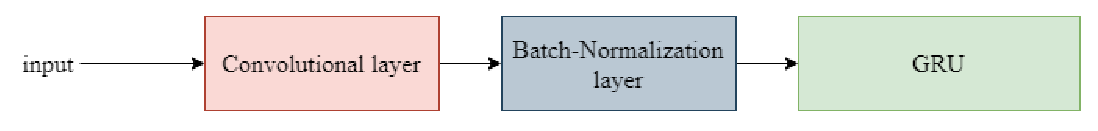
\includegraphics[scale=0.8]{images/gru.eps}
	\captionof{figure}{Schema della rete GRU-C1BN}
	\label{Figura 1.}
\end{center}
\vspace{0.25cm}


\section{Modifica della topologia su rete TCN}
In questa modifica è stato utilizzato un solo livello Convoluzionale inserito subito prima della rete TCN base.

I motivi per cui è stato aggiunto un livello di convoluzione sono gli stessi detti in precedenza: tale livello permette il raggiungimento di una indipendenza spaziale e ciò aiuta il sistema a generalizzare meglio il modello, cosa fondamentale se si vogliono aumentare le performance della rete.
\vspace{0.25cm} 
\begin{center}
	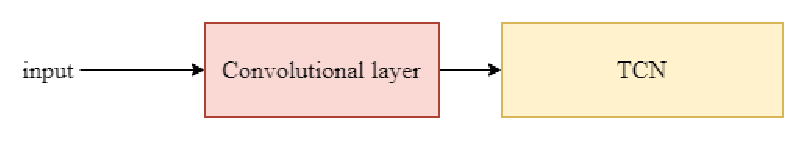
\includegraphics[scale=0.8]{images/tcn.eps}
	\captionof{figure}{Schema della rete TCN-C1}
	\label{Figura 1.}
\end{center}
\vspace{0.25cm}
 % importa il capitolo dal corrispondente file

	% OTTIMIZZATORI -------------------------------------------------------------------------
	\clearpage{\pagestyle{plain}\cleardoublepage} % inizia il nuovo capitolo su di una pagina dispari
	\chapter{Metodi di ottimizzazione} % nome capitolo
	\label{chapter:quarto} % label capitolo
	\addcontentsline{toc}{chapter}{Metodi di ottimizzazione}
	In questo capitolo vengono spiegati i vari metodi di ottimizzazione utilizzati poi negli ensemble.

\section{Metodo Adam}
Adam (Adaptive momentum estimation) è un metodo di ottimizzazione introdotto in [citazione] che calcola il learning rate adattivo per ciascun parametro combinando i concetti di momento e di gradiente adattivo. La regola di aggiornamento si basa sul valore del gradiente al tempo $t$ e sulle medie mobili del gradiente e del suo quadrato. Più precisamente, il metodo Adam definisce le due medie mobili esponenziali (Exponential Moving Average, EMA) $m_{t}$ (primo momento) e $u_{t}$ (secondo momento) come:
\begin{equation}
	m_{t} = \rho_{1}m_{t-1}+(1-\rho_{1})g_{t}
\end{equation}
\begin{equation}
	u_{t} = \rho_{2}u_{t-1}+(1-\rho_{2})g_{t}^{2}
\end{equation}
dove $g_{t}$ è il gradiente al tempo $t$, $g_{t}^{2}$ è il quadrato del gradiente nei termini del quadrato delle sue componenti, $\rho_{1}$ e $\rho_{2}$ sono iper-parametri che rappresentano il tasso di decadimento esponenziale per il primo momento e per il secondo (solitamente settati a 0.9 e 0.999, rispettivamente); inizialmente i momenti sono inizializzati a 0: $m_{t} = u_{t} = 0$. 

Siccome i valori delle due medie mobili potrebbero essere molto piccoli a causa della loro inizializzazione a zero, soprattutto nei primi steps, gli autori del metodo Adam hanno proposto una nuova versione che presenta una correzione ai due momenti:
\begin{equation}
	\hat{m_{t}} = \frac{m_{t}}{(1-\rho_{1}^{t})}
\end{equation}

\begin{equation}
	\hat{u_{t}} = \frac{u_{t}}{(1-\rho_{2}^{t})}
\end{equation}


Infine l'ultimo aggiornamento per ogni parametro $\theta_{t}$ della rete è:

\begin{equation}
	\theta_{t} = \theta_{t-1}-\lambda\frac{\hat{m_{t}}}{\sqrt{\hat{u_{t}}}+\epsilon}
\end{equation}

dove $\lambda$ è il learning rate, $\epsilon$ è un numero positivo molto piccolo in modo tale da prevenire una possibile divisione per 0 (solitamente $\epsilon=10^{-8}$).

\section{Metodo diffGrad}
diffGrad è un metodo di ottimizzazione introdotto in (citazione) che tiene conto della differenza del gradiente per regolare il learning rate.

Si può osservare che quando i cambiamenti del gradiente si riducono durante l'addestramento allora ciò è spesso indicativo della presenza di minimi globali, diffGrad applica una regolazione adattiva data dalla differenza tra il gradiente al tempo $t$ e quello immediatamente passato $t-1$ in modo tale da impostare i parametri nel minimo globale. Pertanto la dimensione del learning rate sarà alta per modifiche repentine del gradiente e bassa per modifiche più lente e graduali.

Per poter definire la regola di aggiornamento occorre determinare il valore assoluto della differenza del gradiente in due istanti di tempo consecutivi:
\begin{equation}
	\Delta g_{t} = |g_{t-1}-g_{t}|
\end{equation}

Infine l'ultimo aggiornamento da effettuare per ogni parametro $\theta_{t}$ della rete è simile all'equazione [5.5], dove $\hat{m_{t}}$, $\hat{u_{t}}$ sono definite come in [5.3], e [5.4] e il learning rate è modulato dalla sigmoide di $\Delta g_{t}$:
\begin{equation}
	\xi_{t} = Sig(\Delta g_{t})
\end{equation}
\begin{equation}
	\theta_{t+1} = \theta_{t}-\lambda\cdot\xi_{t}\frac{\hat{m_{t}}}{\sqrt{\hat{u_{t}}}+\epsilon}
\end{equation}
 
\section{Nuovi metodi di ottimizzazione}
Vengono proposte di seguito diverse varianti del metodo di ottimizzazione diffGrad e Adam:
\begin{itemize}
	\item DGrad si basa sulla media mobile dei quadrati dei parametri del gradiente componente per componente;
	\item Cos\#1 è una variante di DGrad basata sull'applicazione di un cyclic learning rate (CLR);
	\item Exp si basa sull'applicazione di una funzione esponenziale;
	\item Sto è un approccio stocastico per settare il learning rate, che ha lo scopo di evitare che l'ottimizzatore vada in stallo in caso di una zona piatta (plateau).
\end{itemize}
Le varianti proposte differiscono nella definizione del parametro $\xi_{t}$, mentre ciascuna utilizza l'equazione [5.8] nell'aggiornamento finale dei parametri $\theta_{t}$. 

\textbf{DGrad} riprende le idee di diffGrad ri-definendo il valore assoluto della differenza del gradiente in due istanti di tempo consecutivi:
\begin{equation}
	\Delta ag_{t} = | g_{t}-avg_{t} | 
\end{equation}
dove $avg_{t}$ è la media mobile del quadrato, componente per componente, dei parametri del gradiente; poi normalizziamo $\Delta ag_{t}$ con il suo massimo e otteniamo:
\begin{equation}
	\Delta\hat{ag_{t}} = \left(\frac{\Delta ag_{t}}{max(\Delta ag_{t})} \right)
\end{equation}
e definiamo $\xi_{t}$ come:
\begin{equation}
	\xi_{t} = Sig(4 \cdot \Delta \hat{ag_{t}})
\end{equation}
dove il fondamento logico che porta a moltiplicare per "4" l'argomento della funzione sigmoidea è aumentare l'intervallo di output della funzione stessa.

\textbf{Cos\#1} è una variante di DGrad che sfrutta l'idea di utilizzare un learning rate ciclico, con l'obiettivo di migliorare l'accuratezza della classificazione senza tuning e con meno iterazioni [citazione].
Occorre utilizzare una funzione periodica per definire l'intervallo di variazione del learning rate. In questo caso è stata utilizzata la funzione coseno $\cos()$, definita come segue:
\begin{equation}
	lr_{t} = \left(2-\left\lvert\cos\left(\frac{\pi \cdot t}{steps}\right)\right\rvert e^{-0.01 \cdot (mod(t,steps)+1)}\right)
\end{equation}
dove la funzione $mod()$ denota la funzione modulo e il periodo è definito da $steps=30$.

\vspace{0.25cm} 
\begin{center}
	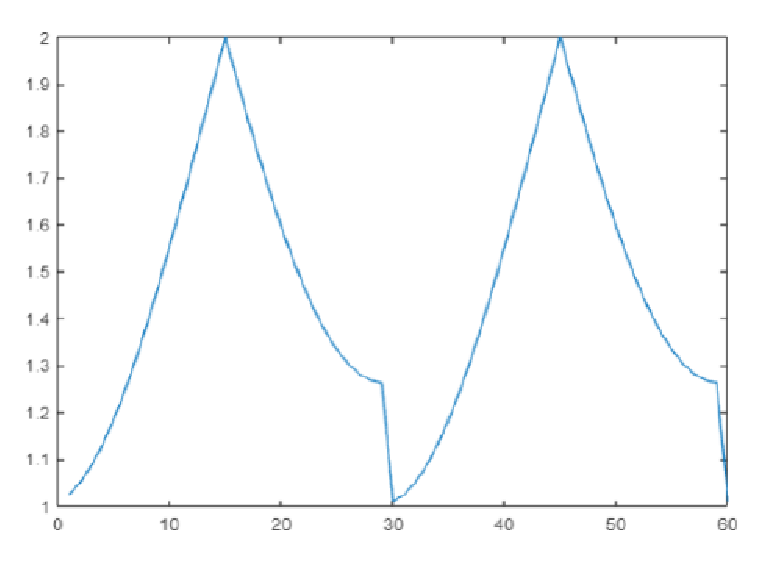
\includegraphics[scale=0.5]{images/clr.eps} %correggere GRU(H UNITA' nascoste)
	\captionof{figure}{Cyclic learning rate}
	\label{Figura 1.}
\end{center}
\vspace{0.25cm}

In questa variante $lr_{t}$ è utilizzato come fattore moltiplicativo di $\hat{ag_{t}}$ nella definizione di $\xi_{t}$, che diventa:
\begin{equation}
	\xi_{t} = Sig(4 \cdot lr_{t} \cdot \Delta \hat{ag_{t}})
\end{equation}


\textbf{Exp} consiste in due semplici operazioni quali prodotto ed esponenziale. Lo scopo di questa variante è di limitare l'effetto di grandi variazioni del gradiente, ma anche di consentire alla funzione di convergere per piccoli valori. L'equazione (18) ha un andamento che decade più lentamente dell'esponenziale negativo per alti valori e, grazie alla normalizzazione, dà meno attenzione alle variazioni del gradiente che tendono a zero, aumentando l'area di maggior guadagno:
\begin{equation}
	lr_{t} = \Delta ag_{t} \cdot e^{-2\cdot\Delta ag_{t}}
\end{equation}

Il parametro $\xi_{t}$ è dato dalla normalizzazione del precedente learning rate per il suo massimo, moltiplicato per "1.5", che aiuta a spostare la media verso l'unità.
\begin{equation}
	\xi_{t} = 1.5 \cdot \frac{lr_{t}}{\max(lr_{t})}
\end{equation}

\vspace{0.25cm} 
\begin{center}
	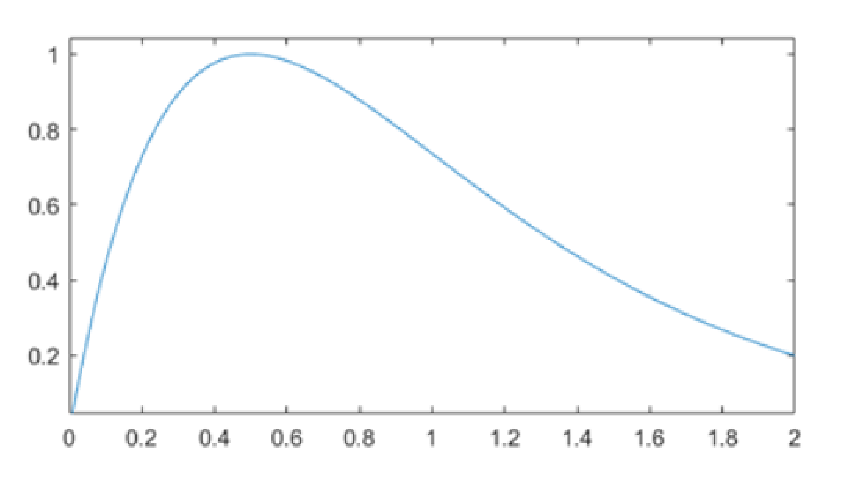
\includegraphics[scale=0.5]{images/exp.eps} %correggere GRU(H UNITA' nascoste)
	\captionof{figure}{Plot dell'eq. 5.14}
	\label{Figura 1.}
\end{center}
\vspace{0.25cm}


\textbf{Sto} è una variante progettata per ridurre la possibilità che l'ottimizzatore possa andare in stallo su zone piatte aggiungendo rumore gaussiano bianco additivo (Additive White Gaussian Noise, AWGN) al learning rate. Il rumore additivo è indipendente dalla direzione del gradiente, quindi aggiunge un certo grado di incertezza alla ricerca dell'ottimo e potrebbe aiutare a trovare il minimo locale quando l'ottimizzatore fa fatica a causa di un learning rate troppo grande.

Sia $X$ una matrice di variabili casuali uniformi e indipendenti nell'intervallo $[0,1]$ e $J$ una matrice di tutti "1":
\begin{eqnarray*}
	\mathcal{X} =
	\begin{bmatrix}
		X_{1,1} & \cdots & X_{1,n}\\
		\vdots & \ddots & \vdots\\
		X_{m,1} & \cdots & X_{m,n}
	\end{bmatrix}
	\hspace{45pt}
	J = 
	\begin{bmatrix}
		1 & \cdots & 1\\
		\vdots & \ddots & \vdots\\
		1 & \cdots & 1
	\end{bmatrix}
\end{eqnarray*}
dove $X_{i,j} \sim \mathcal{U}(0,1)$ sono variabili casuali con funzione di densità di probabilità uniforme. Il learning rate è definito come:

\begin{equation}
	lr_{t} = \Delta ag_{t} \cdot e^{(-4\cdot\Delta ag_{t})} \cdot (\mathcal{X} + 0.5 \cdot J)
\end{equation}
dunque
\begin{equation}
	\xi_{t} = 1.5 \cdot \frac{lr_{t}}{\max(lr_{t})}
\end{equation}

Nell'eq. 20 la matrice $J$ viene utilizzata per shiftare l'intervallo di $X$ di 0.5 per spostare la media su 1.
 % importa il capitolo dal corrispondente file

	% RIS. SPERIMENTALI -------------------------------------------------------------------------
	\clearpage{\pagestyle{plain}\cleardoublepage} % inizia il nuovo capitolo su di una pagina dispari
	\chapter{Risultati sperimentali} % nome capitolo
	\label{chapter:quinto} % label capitolo
	\addcontentsline{toc}{chapter}{Risultati sperimentali}
	risultati



convluzione porta a genenralizzare meglio il problkema e blablabla, bathc rende più stabile ila rete e bla bla bla % importa il capitolo dal corrispondente file
	
	% CONCLUSIONI -------------------------------------------------------------------------
	\clearpage{\pagestyle{plain}\cleardoublepage} % inizia il nuovo capitolo su di una pagina dispari
	\chapter{Conclusioni} % nome capitolo
	\label{chapter:sesto} % label capitolo
	\addcontentsline{toc}{chapter}{Conclusioni}
	\input{conclusioni.tex} % importa il capitolo dal corrispondente file

	% BIBLIOGRAFIA ------------------------------------------------------
	\pagestyle{plain}
	\cleardoublepage
	\chapter*{Bibliografia} % nome capitolo
	\addcontentsline{toc}{chapter}{Bibliografia}
	\printbibliography[heading=none]

\end{document}